\subsection*{Inference of an Anopheles recombination atlas}

Previous work inferred recombination maps for populations of \textit{Anopheles gambiae} and \textit{Anopheles coluzzii} using LDhat \citep{nelson2021anopheles}. Other studies have produced chromosome-scale linkage maps and broad recombination patterns in mosquitoes from crosses, including microsatellite maps for \textit{Anopheles gambiae} and \textit{Anopheles funestus}, a RAD-based linkage map for \textit{Aedes aegypti}, and an \textit{Anopheles} saltwater-tolerance QTL map \citep{zheng1996anopheles,wondji2005funestus,juneja2014aedes,smith2015anopheles}. To the best of our knowledge, these resources do not provide population-resolved, genome-wide recombination maps inferred from LD at tens-of-kilobases resolution.

We applied the same fixed atlas model to Phase 2 AR1 phased haplotypes \citep{malariagen_phase2_ar1_2017,ag1000g2020}. The release comprises 1,142 wild mosquitoes from 13 countries. Our primary atlas contains \PhaseTwoCohortCount{} established species-by-population cohorts: \PhaseTwoGambiaeCount{} \Agambiae and \PhaseTwoColuzziiCount{} \Acoluzzii cohorts. We selected exactly 40 diploid mosquitoes per cohort from the intersection of samples represented on all five chromosome arms, giving \PhaseTwoDiploidCount{} mosquitoes in the atlas. Each population map was summarized in nonoverlapping 50-kb windows on 2R, 2L, 3R, 3L, and X (Fig.~\ref{fig:anopheles}A).

The maps show shared chromosome-scale structure as well as population-specific variation. Vertical differences between tracks should not be interpreted as meiotic rate differences because conversion from population-scaled rate is conditional on a population-level estimate of effective population size. Tests of 2La and resistance regions therefore use within-population ratios.

For 2La, we divided the median rate inside the established 20.524--42.166-Mb breakpoints by the median over the remainder of 2L and defined suppression depth as \(1-r_{\mathrm{in}}/r_{\mathrm{out}}\). Arrangement frequency was estimated from all released mosquitoes in each cohort using \PhaseTwoTagSnpCount{} matched tag SNPs. Across the nine cohorts, suppression depth was positively but imprecisely associated with expected heterokaryotype frequency (Pearson \(r=\PhaseTwoPearsonR\), \(P=\PhaseTwoPearsonP\); Spearman \(r_s=\PhaseTwoSpearmanR\), \(P=\PhaseTwoSpearmanP\); Fig.~\ref{fig:anopheles}B,C). The Phase 2 result is therefore compatible with the predicted relationship but does not establish it statistically.

\subsection*{Released Phase 2 crosses provide a broad-scale comparison}

We next compared the inferred recombination-map consensus with crossovers inferred from the \PhaseTwoCrossCount{} laboratory crosses released with Phase 2. All crosses were included; there is no Phase 2 analogue of a site-filter-held-out family test. The released cross input consists of statistically phased SHAPEIT haplotypes rather than the genotype-quality and explicit site-filter arrays available in later resources. We therefore treat this as a release-specific broad-scale comparison, not as a replication of the later pedigree design.

An atlas-blind two-state caller retained \PhaseTwoCrossoverCount{} autosomal breakpoint intervals no wider than 1 Mb from \PhaseTwoProgenyCount{} progeny. Across \PhaseTwoPedigreeWindowCount{} supported 5-Mb windows, the chromosome-arm-normalized direct and inferred recombination maps had Spearman \(r_s=\PhaseTwoPedigreeR\) (\(P=\PhaseTwoPedigreeP\); Fig.~\ref{fig:phase2-pedigree}). This endpoint tests broad spatial ordering only; it does not validate absolute scale, individual 50-kb windows, or resistance regions.

\begin{figure*}[!t]
\centering
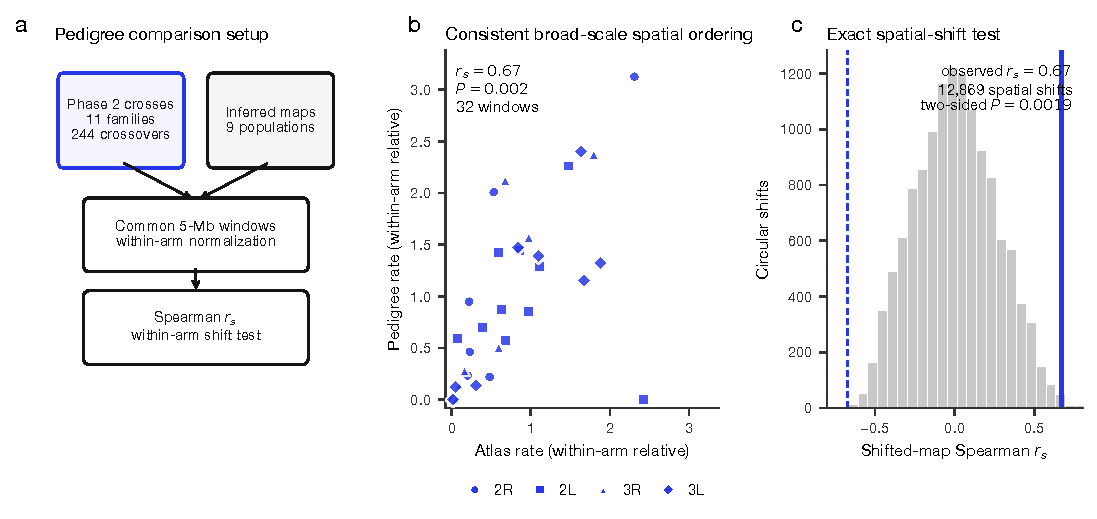
\includegraphics[width=\textwidth]{figures/fig_phase2_pedigree.pdf}
{\captionsetup{labelformat=empty}\caption{\textbf{Figure 4: Broad-scale comparison with the released Phase 2 crosses.} (a) The direct map uses all 11 released crosses (212 progeny and 244 autosomal crossover intervals no wider than 1 Mb), while the inferred recombination-map consensus combines nine wild populations. Both maps were normalized within arm before comparison in common 5-Mb windows. (b) Chromosome-arm-normalized rates in 32 supported autosomal windows. Marker shapes denote chromosome arms; the statistic is a two-sided Spearman correlation. (c) Exact null distribution from all 12,869 nonzero combinations of whole-window circular shifts within chromosome arms. Solid and dashed cobalt lines mark the observed correlation and its negative counterpart, respectively. Calls use the released SHAPEIT representation and are interpreted only at broad resolution.}\label{fig:phase2-pedigree}}
\end{figure*}

\subsection*{Resistance regions are compared with haplotype-matched controls}

The 15 predefined resistance regions were \textit{Vgsc/kdr}, \textit{Rdl}, \textit{Ace1}, \textit{Gste2}, \textit{Cyp6aa/Cyp6p}, \textit{Cyp9k1}, \textit{Cyp4j5}, \textit{Coeae1d}, \textit{Cyp6m2}, \textit{SAP2}, \textit{Cyp4g16}, \textit{Cyp4g17}, \textit{Gstd1}, \textit{Maf-S}, and the adjacent \textit{D7r2}/\textit{D7r4} region. Within each population, focal rates were compared with up to 75 same-arm controls matched on chromosome position, SNP density, nucleotide diversity, and H12; every focal region was excluded from all control pools.

Across the nine populations, the median focal-to-control ratio for the 15 predefined resistance regions was \PhaseTwoResistanceRatio{}, with nominal within-population permutation \(P<0.05\) in \PhaseTwoResistanceSignificantCount{} of \PhaseTwoResistancePopulationCount{} cohorts (Fig.~\ref{fig:anopheles}D,E). The species-stratified median ratio was \PhaseTwoGambiaeResistanceRatio{} in \Agambiae and \PhaseTwoColuzziiResistanceRatio{} in \Acoluzzii. Despite variation among regions and cohorts, resistance-associated regions had lower inferred recombination overall, although this reduction was not observed at every region.

\begin{figure*}[!t]
\centering
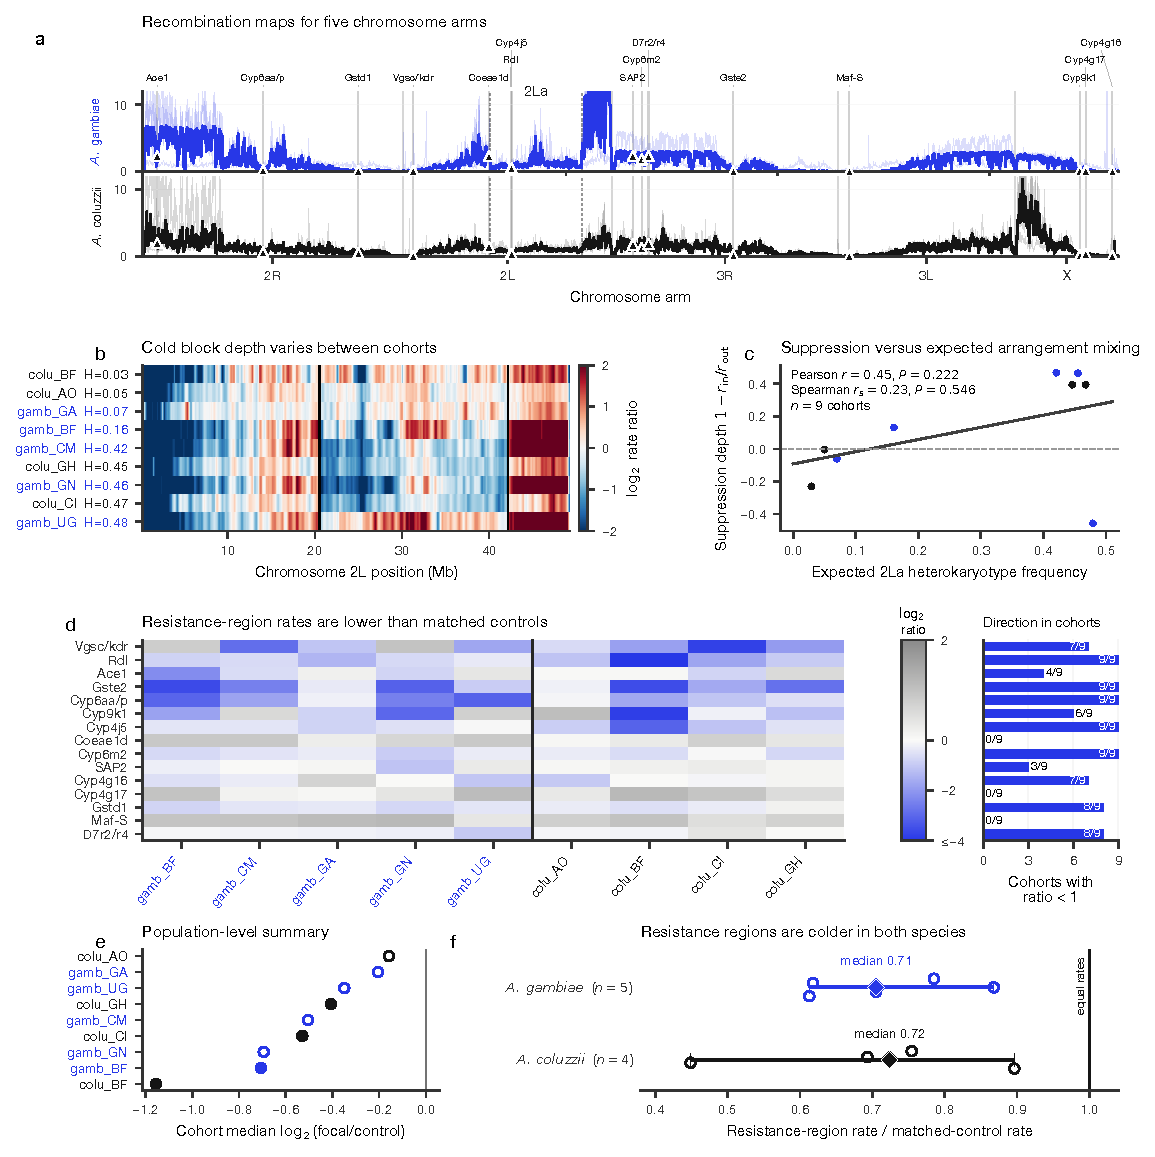
\includegraphics[width=0.97\textwidth,height=0.78\textheight,keepaspectratio]{figures/fig_phase2_anopheles.pdf}
\caption{\textbf{Recombination maps of populations of mosquitoes transmitting malaria.} (a) Phase 2 recombination profiles for nine populations across five chromosome arms. Thin lines show population maps, thick lines show species medians, and triangles mark the 15 predefined resistance regions. Rates are normalized within each chromosome arm for display. (b) Log$_2$ recombination rate along 2L relative to the median rate outside the established 2La breakpoints; tracks are smoothed for presentation. (c) Suppression depth plotted against expected 2La heterokaryotype frequency. Statistics use unsmoothed 100-kb rates and two-sided Pearson and Spearman tests. (d) Log$_2$ focal-to-haplotype-matched-control ratios for each resistance region and cohort; the margin indicates the number of cohorts in which the ratio was below one. (e) Population-level summaries across all 15 resistance regions. Filled symbols indicate descriptive within-population permutation values below 0.05. (f) Population-level median focal-to-control ratios across the 15-region panel (circles), stratified by species. Diamonds show species medians, and error bars show 95\% bootstrap percentile intervals from 4,000 resamples of populations within each species. The reference line at one indicates equal focal and matched-control rates.}\label{fig:anopheles}
\end{figure*}
